\chapter{Robot simulation}
    The robot design is based on the quadristable joint described in the previous chapter. To be more precise, each leg is a multistable joint. As there is different sequences for each leg, the motion of the robot is hard to predict. The structure of the robot will first be described before discussing the actuation of the legs. Finally a section will cover the displacement of the legs and how they interact with the ground.
    
    \begin{figure}[h!]
        \centering
        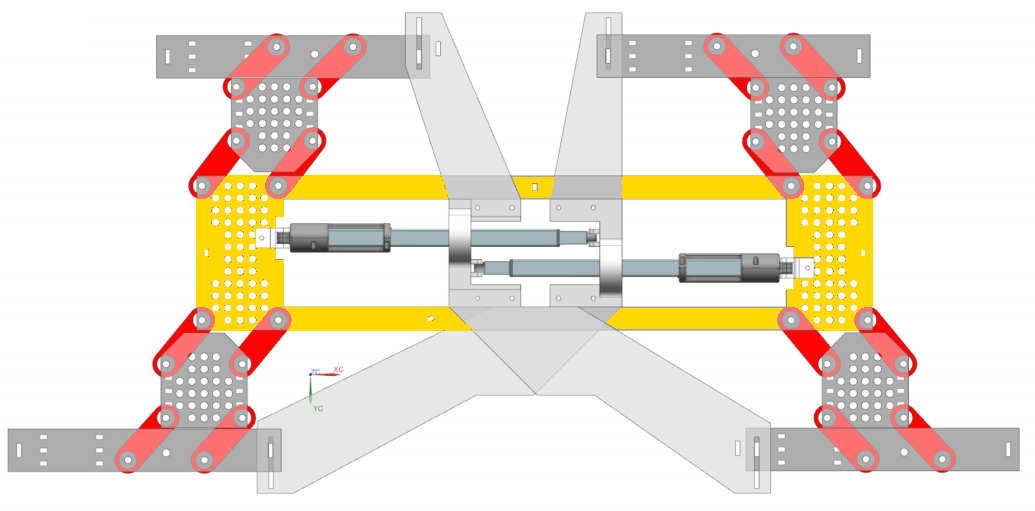
\includegraphics[width=0.8\textwidth]{images/top_view_robot.png}
        \caption{Top view of the robot. There is four identical multistable joints that act as legs. The yellow part is the main frame. This main frame is connecting the ground block of the four quadristable joints together. }
        \label{fig:robot_top_view}
    \end{figure}
    
    \section{Robot structure}
        Figure \ref{fig:robot_top_view} shows a top view of the robot's structure. Each multistable joint also consists of three blocks linked by red arms. The main frame is the yellow part on the schematic, it links the bottom block of the four multistable joints together, this means that the position of the four bottom blocks are static relative to each other. 
        
        
        The legs are an extension of the quadristable joint. The end points of the legs are attached to the middle and the top block of each joint. The way they move will be described the section \ref{sec:legs}. Two actuators are attached on one side to the main yellow frame. They are aligned in the same orientation but they are looking at opposite direction, meaning that if both actuators are extending, the first actuator is extending to the left, while the other is extending to the right.
        
        
        \begin{figure}[h!]
            \centering
            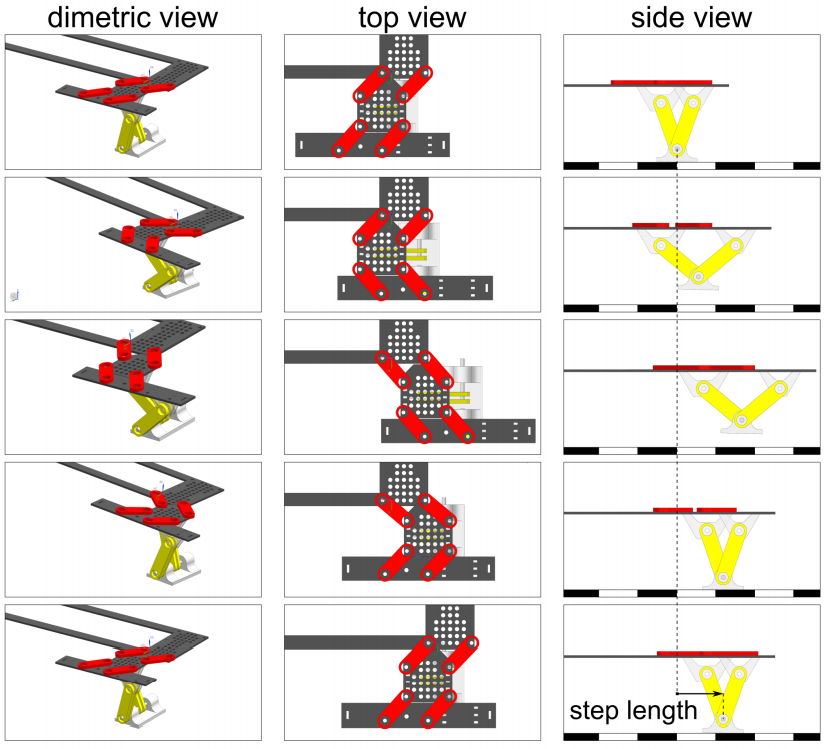
\includegraphics[width=0.8\textwidth]{images/forward_step.png}
            \caption{Specific focus on a leg of a robot, here in sequence B, where the top block moves before the middle block both in forward and backward motion. The leg is attached to a multistable joint and consists of a two arms linking the top block to the middle block with a common pivot. We can see three columns, the first is a dimetric view of the leg, where we can have a 3D view during the cycle. The second represents a top view of the leg that shows how the blocks move in the sequence order. Finally, the third column is a side view of the leg with the two arms and the end plate. It shows how the legs is moving horizontally and vertically. The leg's hysteresis is shown from the robot's frame position.}
            \label{fig:forward_step}
        \end{figure}
        
    \section{Robot legs}\label{sec:legs}
        Legs are connected directly to a multistable joint system. They are right underneath the middle and the top block of the joint. Figure \ref{fig:forward_step} shows a side view, a top view and a dimetric view of a the leg during a cycle. 
        The leg is built with two arms that are connected together on one end and respectively connected to the middle block and the top block on the other ends. This forms a triangular shape as we can see on the side view of Figure \ref{fig:forward_step}. The position of the end of the leg in contact with the ground will be affected by the positions of the middle and the top block. The distance between the two blocks will affect the heights of the end of the leg. Figure's cycle shows that when both blocks translate horizontally together, the end of the leg is moving with them. On the other hand, when the top block moves alone, it will affect not only the horizontal position of the end of the leg, but will also change the height of the leg. Due to the different sequences, the leg pattern may in specific cases draw a hysteresis. This hysteresis is important as it allows the robot to move in different directions depending on the actuation and the sequences selected for the joint. 
        
    \section{Robot actuation}\label{sec:actuation}
        Actuation is performed with linear actuators that are connected to the legs in a specific way. First as shown on Figure \ref{fig:robot_top_view} that they are aligned in the same axis but they are facing opposite direction. They are actuated separately and a phase difference can be defined. A phase difference is $0°$ when when both actuators extend and retract at the same time and at the same speed. A phase difference of $180°$ will occur when one actuator is extending while the other is retracting. As there is two actuators and four legs. Each actuator will be connected to two legs that are in diagonal in the robot view. As seen on Figure \ref{fig:legs_connection}, there are two groups of legs, the green group includes legs one and four and is linked to the first actuator. The second group is the magenta group and includes legs two and three that are linked to the second actuator. 
        
        \begin{figure}
            \centering
            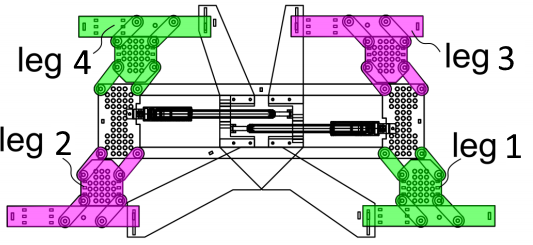
\includegraphics[width=0.5\textwidth]{images/legs_connection.png}
            \caption{Legs connection to the actuators, there are two groups, green groups consists of legs 1 and legs 4, they are connected to one actuator. This means that the top block of each multistable joint will move in coordination with this actuator in the horizontal axis. The second group consists of magenta blocks (legs 2 and legs 3) and are linked to the second actuator.}
            \label{fig:legs_connection}
        \end{figure}